\chapter{Finite Size Scaling Effect}

Recalling Section \ref{sec:stats}, the finite size scaling law hypothesizes that the tail behaviour relates to the finite lattice size $L$ via a probability mass function of the form:
\[p(X=x; \tau, L, f, D) \propto x^{-\tau} f\left(\frac{x}{L^D}\right)\]
Here $f$ governs the tail behaviour of the distribution, i.e. for small values of $u$, $f(u) \approx 1$ and the distribution resembles a power law.

\section{Exponentially Truncated Power Law}
We first consider the exponentially-truncated power law:
\begin{align*}
    p(X=x; \tau, c, x_{max}) &= \frac{1}{C_{\tau, c, x_{max}}} x^{-\tau} \exp\left( \frac{-x}{c} \right) \\
    \intertext{Where $C_{\tau, c, x_{max}}$ is the normalising constant:}
    C_{\tau, c, x_{max}} &= \sum_{k=1}^{x_{max}} k^{-\tau} \exp\left( -k / c \right) \\
\end{align*}

In the above pmf, $\tau$ and $x_{max}$ are, as before, the power law scaling coefficient and the support upper bound respectively, while the new parameter $c$ controls the location of the soft cutoff, where power law behaviour decays.

The shape of the pmf under varying parameter values can be observed in Figure \ref{fig:exp_powerlaw_params}


\begin{figure}
\begin{center}
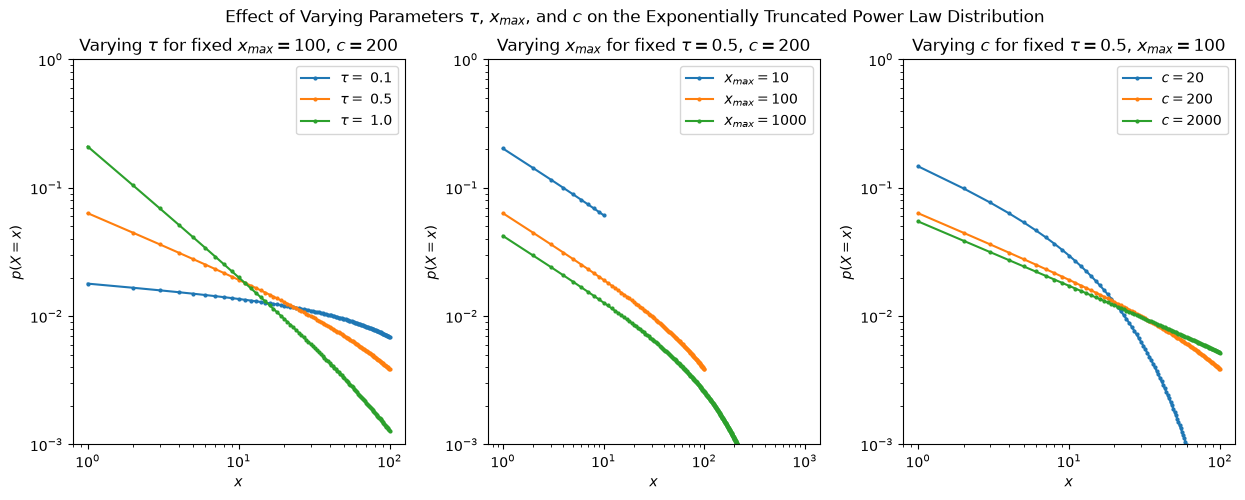
\includegraphics[width=0.80\linewidth]{figures/exp_powerlaw_params.png}
\end{center}
\caption{Visualisation of the exponentially truncated power law probability mass function on log-log axes under different parameter combinations. Each point represents a discrete value and corresponding probability mass, with a line connecting sequential points for illustration purposes. The left plot shows the effect of varying $\tau$ while keeping $x_{max}$ and $c$ constant, which results in changes to the slope of the linear part of the connecting line. The central plot shows the effect of varying $x_{max}$ while keeping $\tau$ and $c$ constant, which results in vertical translation of the connecting curve, with different support for $x$. The right plot shows the effect of increasing $c$ while keeping $\tau$ and $x_{max}$ constant, which results in later decay.The orange line is identical in all plots, corresponding to parameters $\tau = 0.5$, $x_{max} = 100$, and $c = 200$.}
\label{fig:exp_powerlaw_params}
\end{figure} 

The likelihood and log-likelihood are:
\begin{align*}
    \mathcal{L}(\mathbf{x}; \tau, c, x_{max}) &= \prod_{i=1}^n \frac{1}{C_{\tau, c, x_{max}}} x_i^{-\tau} \exp\left( \frac{-x_i}{c} \right) \\
    \log \mathcal{L}(\mathbf{x}; \tau, c, x_{max}) &= -n \log C_{\tau, c, x_{max}} -\tau \sum_{i=1}^T \log x_i - \frac{1}{c}\sum_{i=1}^T x_i \\
\end{align*}

In the above, we model $f(u) = \exp(-u)$. We expect $c_a \propto L^D$ for some constant $D$ across all lattice sizes.
The advantage of this structure is that the full (not truncated) dataset can be used to fit the powerlaw exponent $\tau_a$, with $c_a$ representing a soft cutoff boundary that is fit to the data, rather than a hard cutoff that is chosen arbitrarily.
If the distribution obeys finite size scaling with this $f$, then we should expect to see a relatively constant $\tau_a$ across varying $L$, and we should observe a linear $\log(c_a)$ vs $\log(L)$ plot with constant slope $D_a$.
In particular, we can estimate pooled MLEs from the full dataset across different values of $L$ according to 
\[p(a; L, \tau_a, \gamma_a, D_a) = \frac{1}{C_{L, \tau_a, \gamma_a, D_a}} a^{-\tau_a} \exp\left( \frac{a}{\gamma_a L ^{D_a}} \right)\]

Denote $\mathbf{a}_L$ the set of observations generated from the lattice of size $L$. Then likelihood and log-likelihood in the pooled case are:
\begin{align*}
    \mathcal{L}(\mathbf{a}_{L_1}, \cdots \mathbf{a}_{L_K}; \tau_a, \gamma_a, D_a) &= \prod_{j=1}^K \mathcal{L}(\mathbf{a}_{L_j}; \tau_a, c_a=\gamma_a L_j ^{D_a}, a_{max} = L^2)  \\
\end{align*}


We follow the below procedure:
\begin{enumerate}
    \item For each $L$, estimate MLE parameters $\hat{\tau}_a (L), \hat{c}_a (L)$.
    \item Examine the MLE fit against the observed data
    \item Pool the data and estimate MLE parameters $\tau_a, \hat{gamma}_a, \hat{D}_a$.
    \item Examine the MLE fit of $\log \hat{\gamma}_a, \hat{D}_a$ against $\log \hat{c}_a (L)$ and $\log L$.
\end{enumerate}

\subsection{Estimating MLE parameters for each $L$}
As before, for each $L$, we numerically optimise the log-likelihood function to obtain:
\[\hat{\tau}_a(L), \hat{c}_a(L) = \argmin_{\tau_a, c_a}\left\{ -\log \mathcal{L}(\mathbf{a}_L; \tau_a, c_a, a_{max}=L^2) \right\}\]

\begin{figure}[htbp]
    \centering

    % Left: Figure
    \begin{minipage}[c]{0.48\textwidth}
        \centering
        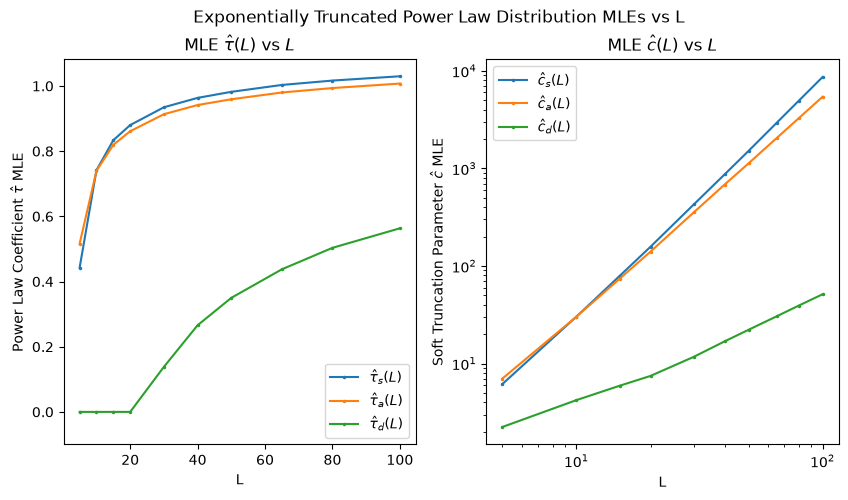
\includegraphics[width=\linewidth]{figures/powerlaw_exp_taus_taua_plot.png}
        \captionof{figure}{Estimates MLEs for $\tau_s, \tau_a$ for varying lattice sizes $L$.}
        \label{fig:powerlaw_exp_taus}
    \end{minipage}
    \hfill
    % Right: Table
    \begin{minipage}[c]{0.48\textwidth}
        \centering
        
        \begin{tabular}{|l|l|l|l|l|}
        \hline
        $L$ & $\tau_s$ & $c_s$ & $\tau_a$ & $c_a$ \\
        \hline
            5 &  0.38 &  5.69 &  0.44 &  6.27 \\
            10 &  0.68 &  27.49 &  0.67 &  26.58 \\
            15 &  0.84 &  81.55 &  0.82 &  74.76 \\
            20 &  0.90 &  169.69 &  0.88 &  148.70 \\
            30 &  0.94 &  444.13 &  0.91 &  355.15 \\
            40 &  0.96 &  902.92 &  0.94 &  671.42 \\
            50 &  0.99 &  1623.38 &  0.96 &  1124.59 \\
            65 &  1.01 &  3237.96 &  0.98 &  2020.08 \\
            80 &  1.02 &  5846.02 &  0.99 &  3306.74 \\
            100 &  1.04 &  10599.48 &  1.01 &  5372.85 \\
        \hline
        \end{tabular}
        \captionof{table}{MLE power-law slopes $\tau$ and soft cutoffs $c$ obtained for varying lattice sizes $L$}
        \label{tab:powerlaw_exp_taus}
    \end{minipage}

\end{figure}

The results in Table \ref{tab:powerlaw_exp_taus} are promising: for lattice sizes 40 and above, the powerlaw coefficient $\tau \approx 1$.
Further, the soft cutoffs $c$ appear to scale appropriately with $L$, a relationship that we will examine in more detail when computing the pooled estimators.


\begin{figure}[!htbp]
\begin{center}
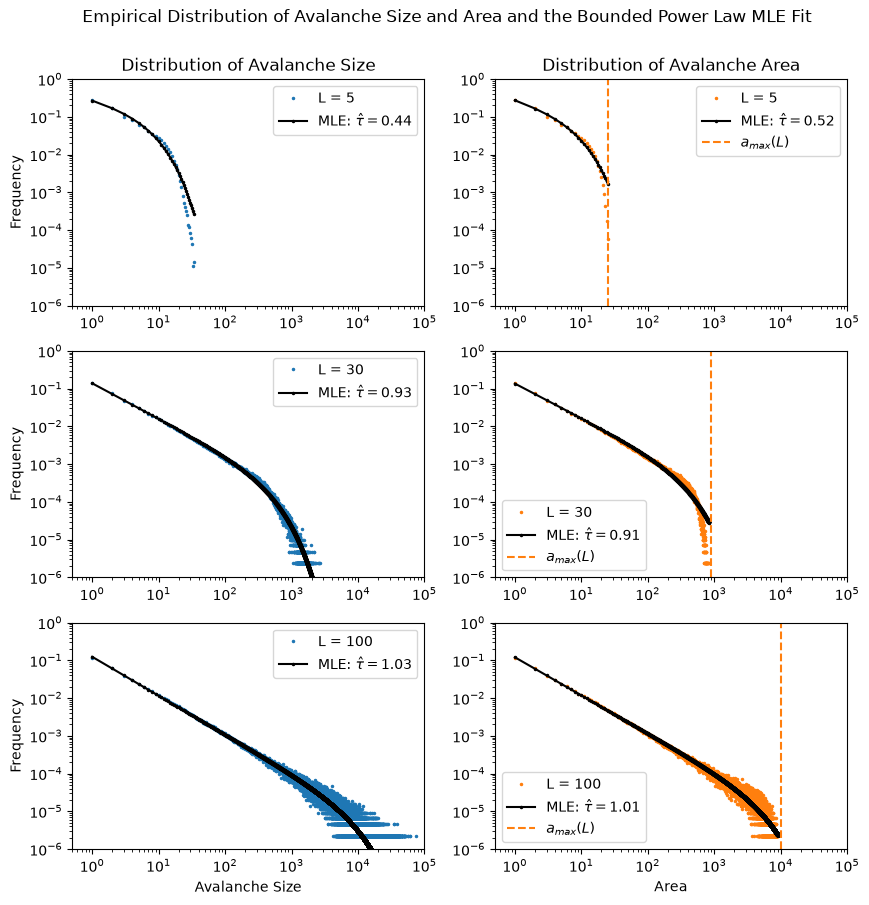
\includegraphics[width=0.80\linewidth]{figures/powerlaw_exp_mle_viz.png}
\end{center}
\caption{Fitted MLEs for the exponentially-truncated power law distribution against the observed data.}
\label{fig:powerlaw_exp_fitted_mle}
\end{figure} 